\documentclass[12pt]{article}
\usepackage[table]{xcolor}
\usepackage{tabularx}
\usepackage{graphicx}
\usepackage{hyperref}
\usepackage{verbatim}
\usepackage{geometry}
\usepackage{ulem}
\usepackage[official]{eurosym}
\usepackage{tikz}
\usetikzlibrary{arrows,backgrounds,calc,decorations.markings,patterns,3d}
\usepackage{pgfplots}
\pgfplotsset{compat = newest}
\usetikzlibrary{fit}
\newcommand\addvmargin[1]{
\usetikzlibrary{arrows}
\node[fit=(current bounding box),inner ysep=#1,inner xsep=0]{};}
\usepackage{cancel}
\usepackage{fontspec}
\usepackage{array}  
\geometry{a4paper, top=2cm, left=2cm, right=2cm, bottom=2cm, headsep=1cm}
\usepackage{tabu}
\usepackage{pst-node}
\usepackage{colortbl}
\usepackage{array}
\usepackage{german}
\setlength\parindent{0pt}
\newcolumntype{?}{!{\vrule width 1pt}}
\usepackage{makecell}
\usepackage{pbox}
\usepackage{amssymb}
\usepackage{amsmath}
\usepackage{booktabs}
\newcolumntype{L}[1]{>{\raggedright\let\newline\\\arraybackslash\hspace{0pt}}m{#1}}
\newcolumntype{C}[1]{>{\centering\let\newline\\\arraybackslash\hspace{0pt}}m{#1}}
\newcolumntype{R}[1]{>{\raggedleft\let\newline\\\arraybackslash\hspace{0pt}}m{#1}}
\begin{document}
\rightline{}
\centerline{{\Large }} 
\vspace{1cm}
\noindent \\


\begin{tabularx}{\textwidth}{|C{1.0cm}|X|}
\arrayrulecolor{black}\hline
a)&{\noindent\begin{tikzpicture}[baseline=0]
\draw[-latex] (0,0) -- (5.5,0) ;
\draw[black] (1.0,0.1) -- (1.0,-0.1) node[below] {$1$} ;
\draw[black] (5.0,0.1) -- (5.0,-0.1) node[below] {$1,1$} ;
\draw[black] (1.0,0.05) -- (1.0,-0.05);
\draw[black] (1.4,0.05) -- (1.4,-0.05);
\draw[black] (1.8,0.05) -- (1.8,-0.05);
\draw[black] (2.2,0.05) -- (2.2,-0.05);
\draw[black] (2.6,0.05) -- (2.6,-0.05);
\draw[black] (3.0,0.05) -- (3.0,-0.05);
\draw[black] (3.4,0.05) -- (3.4,-0.05);
\draw[black] (3.8,0.05) -- (3.8,-0.05);
\draw[black] (4.2,0.05) -- (4.2,-0.05);
\draw[black] (4.6,0.05) -- (4.6,-0.05);
\draw[black] (5.0,0.05) -- (5.0,-0.05);
\draw[-latex] (2.2,0.5) -- (2.2,0.2) ;
\draw (2.2,0.35)node[above] {1,03} ;
\draw[-latex] (1.0,0.75) -- (1.0,0.2) ;
\draw (1.0,0.75)node[above] {1} ;
\end{tikzpicture}
\newline}
\\\hline
\end{tabularx}
\vspace{0.5cm}
\begin{tabularx}{\textwidth}{|C{1.0cm}|X|}
\arrayrulecolor{black}\hline
b)&{\noindent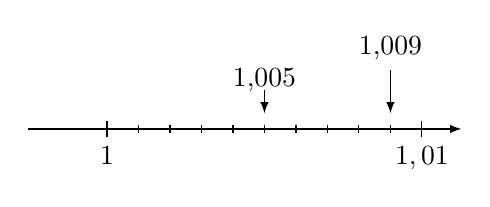
\begin{tikzpicture}[baseline=0]
\draw[-latex] (0,0) -- (5.5,0) ;
\draw[black] (1.0,0.1) -- (1.0,-0.1) node[below] {$1$} ;
\draw[black] (5.0,0.1) -- (5.0,-0.1) node[below] {$1,01$} ;
\draw[black] (0.9999999999999778,0.05) -- (0.9999999999999778,-0.05);
\draw[black] (1.3999999999999333,0.05) -- (1.3999999999999333,-0.05);
\draw[black] (1.7999999999999778,0.05) -- (1.7999999999999778,-0.05);
\draw[black] (2.2000000000000224,0.05) -- (2.2000000000000224,-0.05);
\draw[black] (2.599999999999978,0.05) -- (2.599999999999978,-0.05);
\draw[black] (2.9999999999999334,0.05) -- (2.9999999999999334,-0.05);
\draw[black] (3.3999999999999777,0.05) -- (3.3999999999999777,-0.05);
\draw[black] (3.800000000000022,0.05) -- (3.800000000000022,-0.05);
\draw[black] (4.199999999999978,0.05) -- (4.199999999999978,-0.05);
\draw[black] (4.599999999999933,0.05) -- (4.599999999999933,-0.05);
\draw[black] (4.999999999999978,0.05) -- (4.999999999999978,-0.05);
\draw[-latex] (2.9999999999999334,0.5) -- (2.9999999999999334,0.2) ;
\draw (2.9999999999999334,0.35)node[above] {1,005} ;
\draw[-latex] (4.599999999999933,0.75) -- (4.599999999999933,0.2) ;
\draw (4.599999999999933,0.75)node[above] {1,009} ;
\end{tikzpicture}
\newline}
\\\hline
\end{tabularx}
\vspace{0.5cm}
\begin{tabularx}{\textwidth}{|C{1.0cm}|X|}
\arrayrulecolor{black}\hline
c)&{\noindent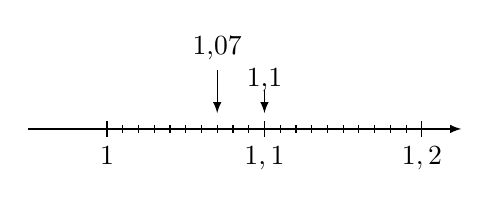
\begin{tikzpicture}[baseline=0]
\draw[-latex] (0,0) -- (5.5,0) ;
\draw[black] (1.0,0.1) -- (1.0,-0.1) node[below] {$1$} ;
\draw[black] (3.0,0.1) -- (3.0,-0.1) node[below] {$1,1$} ;
\draw[black] (5.0,0.1) -- (5.0,-0.1) node[below] {$1,2$} ;
\draw[black] (1.0,0.05) -- (1.0,-0.05);
\draw[black] (1.2,0.05) -- (1.2,-0.05);
\draw[black] (1.4,0.05) -- (1.4,-0.05);
\draw[black] (1.6,0.05) -- (1.6,-0.05);
\draw[black] (1.8,0.05) -- (1.8,-0.05);
\draw[black] (2.0,0.05) -- (2.0,-0.05);
\draw[black] (2.2,0.05) -- (2.2,-0.05);
\draw[black] (2.4,0.05) -- (2.4,-0.05);
\draw[black] (2.6,0.05) -- (2.6,-0.05);
\draw[black] (2.8,0.05) -- (2.8,-0.05);
\draw[black] (3.0,0.05) -- (3.0,-0.05);
\draw[black] (3.1999999999999957,0.05) -- (3.1999999999999957,-0.05);
\draw[black] (3.3999999999999955,0.05) -- (3.3999999999999955,-0.05);
\draw[black] (3.5999999999999956,0.05) -- (3.5999999999999956,-0.05);
\draw[black] (3.7999999999999954,0.05) -- (3.7999999999999954,-0.05);
\draw[black] (3.9999999999999956,0.05) -- (3.9999999999999956,-0.05);
\draw[black] (4.199999999999996,0.05) -- (4.199999999999996,-0.05);
\draw[black] (4.399999999999996,0.05) -- (4.399999999999996,-0.05);
\draw[black] (4.599999999999995,0.05) -- (4.599999999999995,-0.05);
\draw[black] (4.799999999999995,0.05) -- (4.799999999999995,-0.05);
\draw[black] (4.999999999999996,0.05) -- (4.999999999999996,-0.05);
\draw[-latex] (3.0,0.5) -- (3.0,0.2) ;
\draw (3.0,0.35)node[above] {1,1} ;
\draw[-latex] (2.4,0.75) -- (2.4,0.2) ;
\draw (2.4,0.75)node[above] {1,07} ;
\end{tikzpicture}
\newline}
\\\hline
\end{tabularx}
\vspace{0.5cm}
\begin{tabularx}{\textwidth}{|C{1.0cm}|X|}
\arrayrulecolor{black}\hline
a)&{$96,17468>96,17398$}
\\\hline
\end{tabularx}
\vspace{0.5cm}
\begin{tabularx}{\textwidth}{|C{1.0cm}|X|}
\arrayrulecolor{black}\hline
b)&{$1,9842>1,9836$}
\\\hline
\end{tabularx}
\vspace{0.5cm}
\begin{tabularx}{\textwidth}{|C{1.0cm}|X|}
\arrayrulecolor{black}\hline
a)&{\pbox{6cm}{
\tikzstyle{background grid}=[draw, black!15,step=.5cm]
\noindent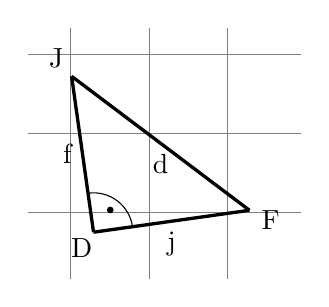
\begin{tikzpicture}[show background grid]
\draw[black, very thick] (-1.980536cm,-0.278346cm) -- node[left] {f} (-1.70219cm,-2.258882cm);
\draw[black, very thick] (-1.70219cm,-2.258882cm) -- node[below] {j} (0.278346cm,-1.980536cm);
\draw[black, very thick] (0.278346cm,-1.980536cm) -- node[below] {d} (-1.980536cm,-0.278346cm);
\node at (-2.176122cm,-0.053377cm) {J};
\node at (-1.852644cm,-2.458541cm) {D};
\node at (0.548511cm,-2.106536cm) {F};
\draw[black] (-1.771776cm,-1.763748cm) arc (98:8:0.5);
\node[circle,draw=black, fill=black, inner sep=0pt,minimum size=2pt] at (-1.489416cm,-1.976522cm) {};
\end{tikzpicture}
\\
$d^2=j^2+f^2$
\\
}}
\\\hline
\end{tabularx}
\vspace{0.5cm}
\begin{tabularx}{\textwidth}{|C{1.0cm}|X|}
\arrayrulecolor{black}\hline
b)&{\pbox{6cm}{
\tikzstyle{background grid}=[draw, black!15,step=.5cm]
\noindent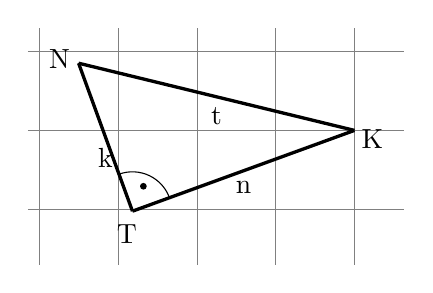
\begin{tikzpicture}[show background grid]
\draw[black, very thick] (0cm,0cm) -- node[below] {t} (-3.503118cm,0.853325cm);
\draw[black, very thick] (-3.503118cm,0.853325cm) -- node[below] {k} (-2.819078cm,-1.02606cm);
\draw[black, very thick] (-2.819078cm,-1.02606cm) -- node[below] {n} (0cm,0cm);
\node at (0.226577cm,-0.105655cm) {K};
\node at (-3.746016cm,0.912492cm) {N};
\node at (-2.89043cm,-1.318075cm) {T};
\draw[black] (-2.349232cm,-0.85505cm) arc (20:110:0.5);
\node[circle,draw=black, fill=black, inner sep=0pt,minimum size=2pt] at (-2.680316cm,-0.709511cm) {};
\end{tikzpicture}
\\
$t^2=n^2+k^2$
\\
}}
\\\hline
\end{tabularx}
\vspace{0.5cm}
\begin{tabularx}{\textwidth}{|C{1.0cm}|X|}
\arrayrulecolor{black}\hline
c)&{\pbox{6cm}{
\tikzstyle{background grid}=[draw, black!15,step=.5cm]
\noindent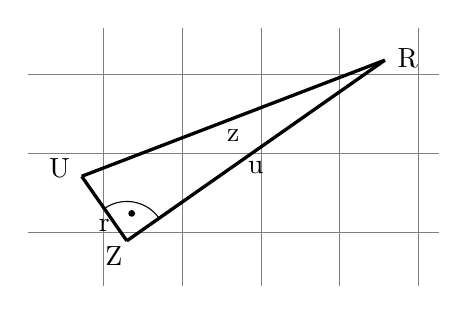
\begin{tikzpicture}[show background grid]
\draw[black, very thick] (-3.276608cm,-2.294306cm) -- node[below] {r} (-2.703032cm,-3.113458cm);
\draw[black, very thick] (-2.703032cm,-3.113458cm) -- node[below] {u} (0.573576cm,-0.819152cm);
\draw[black, very thick] (0.573576cm,-0.819152cm) -- node[below] {z} (-3.276608cm,-2.294306cm);
\node at (-3.558675cm,-2.186617cm) {U};
\node at (-2.866927cm,-3.302239cm) {Z};
\node at (0.864352cm,-0.798561cm) {R};
\draw[black] (-2.98982cm,-2.703882cm) arc (125:35:0.5);
\node[circle,draw=black, fill=black, inner sep=0pt,minimum size=2pt] at (-2.641638cm,-2.765276cm) {};
\end{tikzpicture}
\\
$z^2=u^2+r^2$
\\
}}
\\\hline
\end{tabularx}
\vspace{0.5cm}
\begin{tabularx}{\textwidth}{|C{1.0cm}|X|}
\arrayrulecolor{black}\hline
d)&{\pbox{6cm}{
\tikzstyle{background grid}=[draw, black!15,step=.5cm]
\noindent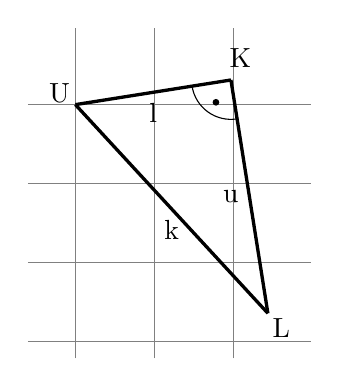
\begin{tikzpicture}[show background grid]
\draw[black, very thick] (0cm,0cm) -- node[below] {k} (2.44468cm,-2.650196cm);
\draw[black, very thick] (2.44468cm,-2.650196cm) -- node[left] {u} (1.975377cm,0.312869cm);
\draw[black, very thick] (1.975377cm,0.312869cm) -- node[below] {l} (0cm,0cm);
\node at (-0.202254cm,0.146946cm) {U};
\node at (2.614188cm,-2.833954cm) {L};
\node at (2.096642cm,0.585192cm) {K};
\draw[black] (1.481533cm,0.234652cm) arc (189:279:0.5);
\node[circle,draw=black, fill=black, inner sep=0pt,minimum size=2pt] at (1.785111cm,0.029618cm) {};
\end{tikzpicture}
\\
$k^2=l^2+u^2$
\\
}}
\\\hline
\end{tabularx}
\vspace{0.5cm}
\begin{tabularx}{\textwidth}{|C{1.0cm}|X|}
\arrayrulecolor{black}\hline
\end{tabularx}
\vspace{0.5cm}
\end{document}